% Start preamble
\documentclass[12pt,a4paper]{article}
\usepackage{geometry}
 \geometry{
 a4paper,
 total={170mm,257mm},
 left=20mm,
 top=20mm,
 }
\usepackage[utf8]{inputenc}
\usepackage[T1]{fontenc}
\usepackage[pdftex]{graphicx}
\graphicspath{{./}}
\usepackage{enumitem}
\usepackage{pdfpages}
\usepackage{hyperref}
\usepackage{tikz}
\usepackage{attachfile}
\usepackage{epstopdf}
\usepackage{array}
%\usepackage[table]{xcolor,colorbl}
\setlength{\textwidth}{16cm}
\setlength{\oddsidemargin}{-0.5cm}
\setlength{\evensidemargin}{-0.5cm}
%\setlenght{\headsep}{0cm}
\setlength\parindent{0pt}
%\setlength{\extrarowheight}{3pt}
\usepackage{listings}
%\usepackage{xcolor}

 %%%%%%%%%%%%%%%%%%%%%%%%%%%%%%%%%%%%%%%%%%%%%%%%%%%%%%%%%%%%%%%%%%%%%%%%%%%%%%%% 
%%% ~ Arduino Language - Arduino IDE Colors ~                                  %%%
%%%                                                                            %%%
%%% Kyle Rocha-Brownell | 10/2/2017 | No Licence                               %%%
%%% -------------------------------------------------------------------------- %%%
%%%                                                                            %%%
%%% Place this file in your working directory (next to the latex file you're   %%%
%%% working on).  To add it to your project, place:                            %%%
%%%     %%%%%%%%%%%%%%%%%%%%%%%%%%%%%%%%%%%%%%%%%%%%%%%%%%%%%%%%%%%%%%%%%%%%%%%%%%%%%%%% 
%%% ~ Arduino Language - Arduino IDE Colors ~                                  %%%
%%%                                                                            %%%
%%% Kyle Rocha-Brownell | 10/2/2017 | No Licence                               %%%
%%% -------------------------------------------------------------------------- %%%
%%%                                                                            %%%
%%% Place this file in your working directory (next to the latex file you're   %%%
%%% working on).  To add it to your project, place:                            %%%
%%%     %%%%%%%%%%%%%%%%%%%%%%%%%%%%%%%%%%%%%%%%%%%%%%%%%%%%%%%%%%%%%%%%%%%%%%%%%%%%%%%% 
%%% ~ Arduino Language - Arduino IDE Colors ~                                  %%%
%%%                                                                            %%%
%%% Kyle Rocha-Brownell | 10/2/2017 | No Licence                               %%%
%%% -------------------------------------------------------------------------- %%%
%%%                                                                            %%%
%%% Place this file in your working directory (next to the latex file you're   %%%
%%% working on).  To add it to your project, place:                            %%%
%%%    \input{arduinoLanguage.tex}                                             %%%
%%% somewhere before \begin{document} in your latex file.                      %%%
%%%                                                                            %%%
%%% In your document, place your arduino code between:                         %%%
%%%   \begin{lstlisting}[language=Arduino]                                     %%%
%%% and:                                                                       %%%
%%%   \end{lstlisting}                                                         %%%
%%%                                                                            %%%
%%% Or create your own style to add non-built-in functions and variables.      %%%
%%%                                                                            %%%
 %%%%%%%%%%%%%%%%%%%%%%%%%%%%%%%%%%%%%%%%%%%%%%%%%%%%%%%%%%%%%%%%%%%%%%%%%%%%%%%% 

\usepackage{color}
\usepackage{listings}    
\usepackage{courier}

%%% Define Custom IDE Colors %%%
\definecolor{arduinoGreen}    {rgb} {0.17, 0.43, 0.01}
\definecolor{arduinoGrey}     {rgb} {0.47, 0.47, 0.33}
\definecolor{arduinoOrange}   {rgb} {0.8 , 0.4 , 0   }
\definecolor{arduinoBlue}     {rgb} {0.01, 0.61, 0.98}
\definecolor{arduinoDarkBlue} {rgb} {0.0 , 0.2 , 0.5 }

%%% Define Arduino Language %%%
\lstdefinelanguage{Arduino}{
  language=C++, % begin with default C++ settings 
%
%
  %%% Keyword Color Group 1 %%%  (called KEYWORD3 by arduino)
  keywordstyle=\color{arduinoGreen},   
  deletekeywords={  % remove all arduino keywords that might be in c++
                break, case, override, final, continue, default, do, else, for, 
                if, return, goto, switch, throw, try, while, setup, loop, export, 
                not, or, and, xor, include, define, elif, else, error, if, ifdef, 
                ifndef, pragma, warning,
                HIGH, LOW, INPUT, INPUT_PULLUP, OUTPUT, DEC, BIN, HEX, OCT, PI, 
                HALF_PI, TWO_PI, LSBFIRST, MSBFIRST, CHANGE, FALLING, RISING, 
                DEFAULT, EXTERNAL, INTERNAL, INTERNAL1V1, INTERNAL2V56, LED_BUILTIN, 
                LED_BUILTIN_RX, LED_BUILTIN_TX, DIGITAL_MESSAGE, FIRMATA_STRING, 
                ANALOG_MESSAGE, REPORT_DIGITAL, REPORT_ANALOG, SET_PIN_MODE, 
                SYSTEM_RESET, SYSEX_START, auto, int8_t, int16_t, int32_t, int64_t, 
                uint8_t, uint16_t, uint32_t, uint64_t, char16_t, char32_t, operator, 
                enum, delete, bool, boolean, byte, char, const, false, float, double, 
                null, NULL, int, long, new, private, protected, public, short, 
                signed, static, volatile, String, void, true, unsigned, word, array, 
                sizeof, dynamic_cast, typedef, const_cast, struct, static_cast, union, 
                friend, extern, class, reinterpret_cast, register, explicit, inline, 
                _Bool, complex, _Complex, _Imaginary, atomic_bool, atomic_char, 
                atomic_schar, atomic_uchar, atomic_short, atomic_ushort, atomic_int, 
                atomic_uint, atomic_long, atomic_ulong, atomic_llong, atomic_ullong, 
                virtual, PROGMEM,
                Serial, Serial1, Serial2, Serial3, SerialUSB, Keyboard, Mouse,
                abs, acos, asin, atan, atan2, ceil, constrain, cos, degrees, exp, 
                floor, log, map, max, min, radians, random, randomSeed, round, sin, 
                sq, sqrt, tan, pow, bitRead, bitWrite, bitSet, bitClear, bit, 
                highByte, lowByte, analogReference, analogRead, 
                analogReadResolution, analogWrite, analogWriteResolution, 
                attachInterrupt, detachInterrupt, digitalPinToInterrupt, delay, 
                delayMicroseconds, digitalWrite, digitalRead, interrupts, millis, 
                micros, noInterrupts, noTone, pinMode, pulseIn, pulseInLong, shiftIn, 
                shiftOut, tone, yield, Stream, begin, end, peek, read, print, 
                println, available, availableForWrite, flush, setTimeout, find, 
                findUntil, parseInt, parseFloat, readBytes, readBytesUntil, readString, 
                readStringUntil, trim, toUpperCase, toLowerCase, charAt, compareTo, 
                concat, endsWith, startsWith, equals, equalsIgnoreCase, getBytes, 
                indexOf, lastIndexOf, length, replace, setCharAt, substring, 
                toCharArray, toInt, press, release, releaseAll, accept, click, move, 
                isPressed, isAlphaNumeric, isAlpha, isAscii, isWhitespace, isControl, 
                isDigit, isGraph, isLowerCase, isPrintable, isPunct, isSpace, 
                isUpperCase, isHexadecimalDigit, 
                }, 
  morekeywords={   % add arduino structures to group 1
                break, case, override, final, continue, default, do, else, for, 
                if, return, goto, switch, throw, try, while, setup, loop, export, 
                not, or, and, xor, include, define, elif, else, error, if, ifdef, 
                ifndef, pragma, warning,
                }, 
% 
%
  %%% Keyword Color Group 2 %%%  (called LITERAL1 by arduino)
  keywordstyle=[2]\color{arduinoBlue},   
  keywords=[2]{   % add variables and dataTypes as 2nd group  
                HIGH, LOW, INPUT, INPUT_PULLUP, OUTPUT, DEC, BIN, HEX, OCT, PI, 
                HALF_PI, TWO_PI, LSBFIRST, MSBFIRST, CHANGE, FALLING, RISING, 
                DEFAULT, EXTERNAL, INTERNAL, INTERNAL1V1, INTERNAL2V56, LED_BUILTIN, 
                LED_BUILTIN_RX, LED_BUILTIN_TX, DIGITAL_MESSAGE, FIRMATA_STRING, 
                ANALOG_MESSAGE, REPORT_DIGITAL, REPORT_ANALOG, SET_PIN_MODE, 
                SYSTEM_RESET, SYSEX_START, auto, int8_t, int16_t, int32_t, int64_t, 
                uint8_t, uint16_t, uint32_t, uint64_t, char16_t, char32_t, operator, 
                enum, delete, bool, boolean, byte, char, const, false, float, double, 
                null, NULL, int, long, new, private, protected, public, short, 
                signed, static, volatile, String, void, true, unsigned, word, array, 
                sizeof, dynamic_cast, typedef, const_cast, struct, static_cast, union, 
                friend, extern, class, reinterpret_cast, register, explicit, inline, 
                _Bool, complex, _Complex, _Imaginary, atomic_bool, atomic_char, 
                atomic_schar, atomic_uchar, atomic_short, atomic_ushort, atomic_int, 
                atomic_uint, atomic_long, atomic_ulong, atomic_llong, atomic_ullong, 
                virtual, PROGMEM,
                },  
% 
%
  %%% Keyword Color Group 3 %%%  (called KEYWORD1 by arduino)
  keywordstyle=[3]\bfseries\color{arduinoOrange},
  keywords=[3]{  % add built-in functions as a 3rd group
                Serial, Serial1, Serial2, Serial3, SerialUSB, Keyboard, Mouse,
                },      
%
%
  %%% Keyword Color Group 4 %%%  (called KEYWORD2 by arduino)
  keywordstyle=[4]\color{arduinoOrange},
  keywords=[4]{  % add more built-in functions as a 4th group
                abs, acos, asin, atan, atan2, ceil, constrain, cos, degrees, exp, 
                floor, log, map, max, min, radians, random, randomSeed, round, sin, 
                sq, sqrt, tan, pow, bitRead, bitWrite, bitSet, bitClear, bit, 
                highByte, lowByte, analogReference, analogRead, 
                analogReadResolution, analogWrite, analogWriteResolution, 
                attachInterrupt, detachInterrupt, digitalPinToInterrupt, delay, 
                delayMicroseconds, digitalWrite, digitalRead, interrupts, millis, 
                micros, noInterrupts, noTone, pinMode, pulseIn, pulseInLong, shiftIn, 
                shiftOut, tone, yield, Stream, begin, end, peek, read, print, 
                println, available, availableForWrite, flush, setTimeout, find, 
                findUntil, parseInt, parseFloat, readBytes, readBytesUntil, readString, 
                readStringUntil, trim, toUpperCase, toLowerCase, charAt, compareTo, 
                concat, endsWith, startsWith, equals, equalsIgnoreCase, getBytes, 
                indexOf, lastIndexOf, length, replace, setCharAt, substring, 
                toCharArray, toInt, press, release, releaseAll, accept, click, move, 
                isPressed, isAlphaNumeric, isAlpha, isAscii, isWhitespace, isControl, 
                isDigit, isGraph, isLowerCase, isPrintable, isPunct, isSpace, 
                isUpperCase, isHexadecimalDigit, 
                },      
%
%
  %%% Set Other Colors %%%
  stringstyle=\color{arduinoDarkBlue},    
  commentstyle=\color{arduinoGrey},    
%          
%   
  %%%% Line Numbering %%%%
%  numbers=left,                    
%  numbersep=5pt,                   
%  numberstyle=\color{arduinoGrey},    
  %stepnumber=2,                      % show every 2 line numbers
%
%
  %%%% Code Box Style %%%%
  breaklines=true,                    % wordwrapping
  tabsize=8,         
  basicstyle=\ttfamily  
}
                                             %%%
%%% somewhere before \begin{document} in your latex file.                      %%%
%%%                                                                            %%%
%%% In your document, place your arduino code between:                         %%%
%%%   \begin{lstlisting}[language=Arduino]                                     %%%
%%% and:                                                                       %%%
%%%   \end{lstlisting}                                                         %%%
%%%                                                                            %%%
%%% Or create your own style to add non-built-in functions and variables.      %%%
%%%                                                                            %%%
 %%%%%%%%%%%%%%%%%%%%%%%%%%%%%%%%%%%%%%%%%%%%%%%%%%%%%%%%%%%%%%%%%%%%%%%%%%%%%%%% 

\usepackage{color}
\usepackage{listings}    
\usepackage{courier}

%%% Define Custom IDE Colors %%%
\definecolor{arduinoGreen}    {rgb} {0.17, 0.43, 0.01}
\definecolor{arduinoGrey}     {rgb} {0.47, 0.47, 0.33}
\definecolor{arduinoOrange}   {rgb} {0.8 , 0.4 , 0   }
\definecolor{arduinoBlue}     {rgb} {0.01, 0.61, 0.98}
\definecolor{arduinoDarkBlue} {rgb} {0.0 , 0.2 , 0.5 }

%%% Define Arduino Language %%%
\lstdefinelanguage{Arduino}{
  language=C++, % begin with default C++ settings 
%
%
  %%% Keyword Color Group 1 %%%  (called KEYWORD3 by arduino)
  keywordstyle=\color{arduinoGreen},   
  deletekeywords={  % remove all arduino keywords that might be in c++
                break, case, override, final, continue, default, do, else, for, 
                if, return, goto, switch, throw, try, while, setup, loop, export, 
                not, or, and, xor, include, define, elif, else, error, if, ifdef, 
                ifndef, pragma, warning,
                HIGH, LOW, INPUT, INPUT_PULLUP, OUTPUT, DEC, BIN, HEX, OCT, PI, 
                HALF_PI, TWO_PI, LSBFIRST, MSBFIRST, CHANGE, FALLING, RISING, 
                DEFAULT, EXTERNAL, INTERNAL, INTERNAL1V1, INTERNAL2V56, LED_BUILTIN, 
                LED_BUILTIN_RX, LED_BUILTIN_TX, DIGITAL_MESSAGE, FIRMATA_STRING, 
                ANALOG_MESSAGE, REPORT_DIGITAL, REPORT_ANALOG, SET_PIN_MODE, 
                SYSTEM_RESET, SYSEX_START, auto, int8_t, int16_t, int32_t, int64_t, 
                uint8_t, uint16_t, uint32_t, uint64_t, char16_t, char32_t, operator, 
                enum, delete, bool, boolean, byte, char, const, false, float, double, 
                null, NULL, int, long, new, private, protected, public, short, 
                signed, static, volatile, String, void, true, unsigned, word, array, 
                sizeof, dynamic_cast, typedef, const_cast, struct, static_cast, union, 
                friend, extern, class, reinterpret_cast, register, explicit, inline, 
                _Bool, complex, _Complex, _Imaginary, atomic_bool, atomic_char, 
                atomic_schar, atomic_uchar, atomic_short, atomic_ushort, atomic_int, 
                atomic_uint, atomic_long, atomic_ulong, atomic_llong, atomic_ullong, 
                virtual, PROGMEM,
                Serial, Serial1, Serial2, Serial3, SerialUSB, Keyboard, Mouse,
                abs, acos, asin, atan, atan2, ceil, constrain, cos, degrees, exp, 
                floor, log, map, max, min, radians, random, randomSeed, round, sin, 
                sq, sqrt, tan, pow, bitRead, bitWrite, bitSet, bitClear, bit, 
                highByte, lowByte, analogReference, analogRead, 
                analogReadResolution, analogWrite, analogWriteResolution, 
                attachInterrupt, detachInterrupt, digitalPinToInterrupt, delay, 
                delayMicroseconds, digitalWrite, digitalRead, interrupts, millis, 
                micros, noInterrupts, noTone, pinMode, pulseIn, pulseInLong, shiftIn, 
                shiftOut, tone, yield, Stream, begin, end, peek, read, print, 
                println, available, availableForWrite, flush, setTimeout, find, 
                findUntil, parseInt, parseFloat, readBytes, readBytesUntil, readString, 
                readStringUntil, trim, toUpperCase, toLowerCase, charAt, compareTo, 
                concat, endsWith, startsWith, equals, equalsIgnoreCase, getBytes, 
                indexOf, lastIndexOf, length, replace, setCharAt, substring, 
                toCharArray, toInt, press, release, releaseAll, accept, click, move, 
                isPressed, isAlphaNumeric, isAlpha, isAscii, isWhitespace, isControl, 
                isDigit, isGraph, isLowerCase, isPrintable, isPunct, isSpace, 
                isUpperCase, isHexadecimalDigit, 
                }, 
  morekeywords={   % add arduino structures to group 1
                break, case, override, final, continue, default, do, else, for, 
                if, return, goto, switch, throw, try, while, setup, loop, export, 
                not, or, and, xor, include, define, elif, else, error, if, ifdef, 
                ifndef, pragma, warning,
                }, 
% 
%
  %%% Keyword Color Group 2 %%%  (called LITERAL1 by arduino)
  keywordstyle=[2]\color{arduinoBlue},   
  keywords=[2]{   % add variables and dataTypes as 2nd group  
                HIGH, LOW, INPUT, INPUT_PULLUP, OUTPUT, DEC, BIN, HEX, OCT, PI, 
                HALF_PI, TWO_PI, LSBFIRST, MSBFIRST, CHANGE, FALLING, RISING, 
                DEFAULT, EXTERNAL, INTERNAL, INTERNAL1V1, INTERNAL2V56, LED_BUILTIN, 
                LED_BUILTIN_RX, LED_BUILTIN_TX, DIGITAL_MESSAGE, FIRMATA_STRING, 
                ANALOG_MESSAGE, REPORT_DIGITAL, REPORT_ANALOG, SET_PIN_MODE, 
                SYSTEM_RESET, SYSEX_START, auto, int8_t, int16_t, int32_t, int64_t, 
                uint8_t, uint16_t, uint32_t, uint64_t, char16_t, char32_t, operator, 
                enum, delete, bool, boolean, byte, char, const, false, float, double, 
                null, NULL, int, long, new, private, protected, public, short, 
                signed, static, volatile, String, void, true, unsigned, word, array, 
                sizeof, dynamic_cast, typedef, const_cast, struct, static_cast, union, 
                friend, extern, class, reinterpret_cast, register, explicit, inline, 
                _Bool, complex, _Complex, _Imaginary, atomic_bool, atomic_char, 
                atomic_schar, atomic_uchar, atomic_short, atomic_ushort, atomic_int, 
                atomic_uint, atomic_long, atomic_ulong, atomic_llong, atomic_ullong, 
                virtual, PROGMEM,
                },  
% 
%
  %%% Keyword Color Group 3 %%%  (called KEYWORD1 by arduino)
  keywordstyle=[3]\bfseries\color{arduinoOrange},
  keywords=[3]{  % add built-in functions as a 3rd group
                Serial, Serial1, Serial2, Serial3, SerialUSB, Keyboard, Mouse,
                },      
%
%
  %%% Keyword Color Group 4 %%%  (called KEYWORD2 by arduino)
  keywordstyle=[4]\color{arduinoOrange},
  keywords=[4]{  % add more built-in functions as a 4th group
                abs, acos, asin, atan, atan2, ceil, constrain, cos, degrees, exp, 
                floor, log, map, max, min, radians, random, randomSeed, round, sin, 
                sq, sqrt, tan, pow, bitRead, bitWrite, bitSet, bitClear, bit, 
                highByte, lowByte, analogReference, analogRead, 
                analogReadResolution, analogWrite, analogWriteResolution, 
                attachInterrupt, detachInterrupt, digitalPinToInterrupt, delay, 
                delayMicroseconds, digitalWrite, digitalRead, interrupts, millis, 
                micros, noInterrupts, noTone, pinMode, pulseIn, pulseInLong, shiftIn, 
                shiftOut, tone, yield, Stream, begin, end, peek, read, print, 
                println, available, availableForWrite, flush, setTimeout, find, 
                findUntil, parseInt, parseFloat, readBytes, readBytesUntil, readString, 
                readStringUntil, trim, toUpperCase, toLowerCase, charAt, compareTo, 
                concat, endsWith, startsWith, equals, equalsIgnoreCase, getBytes, 
                indexOf, lastIndexOf, length, replace, setCharAt, substring, 
                toCharArray, toInt, press, release, releaseAll, accept, click, move, 
                isPressed, isAlphaNumeric, isAlpha, isAscii, isWhitespace, isControl, 
                isDigit, isGraph, isLowerCase, isPrintable, isPunct, isSpace, 
                isUpperCase, isHexadecimalDigit, 
                },      
%
%
  %%% Set Other Colors %%%
  stringstyle=\color{arduinoDarkBlue},    
  commentstyle=\color{arduinoGrey},    
%          
%   
  %%%% Line Numbering %%%%
%  numbers=left,                    
%  numbersep=5pt,                   
%  numberstyle=\color{arduinoGrey},    
  %stepnumber=2,                      % show every 2 line numbers
%
%
  %%%% Code Box Style %%%%
  breaklines=true,                    % wordwrapping
  tabsize=8,         
  basicstyle=\ttfamily  
}
                                             %%%
%%% somewhere before \begin{document} in your latex file.                      %%%
%%%                                                                            %%%
%%% In your document, place your arduino code between:                         %%%
%%%   \begin{lstlisting}[language=Arduino]                                     %%%
%%% and:                                                                       %%%
%%%   \end{lstlisting}                                                         %%%
%%%                                                                            %%%
%%% Or create your own style to add non-built-in functions and variables.      %%%
%%%                                                                            %%%
 %%%%%%%%%%%%%%%%%%%%%%%%%%%%%%%%%%%%%%%%%%%%%%%%%%%%%%%%%%%%%%%%%%%%%%%%%%%%%%%% 

\usepackage{color}
\usepackage{listings}    
\usepackage{courier}

%%% Define Custom IDE Colors %%%
\definecolor{arduinoGreen}    {rgb} {0.17, 0.43, 0.01}
\definecolor{arduinoGrey}     {rgb} {0.47, 0.47, 0.33}
\definecolor{arduinoOrange}   {rgb} {0.8 , 0.4 , 0   }
\definecolor{arduinoBlue}     {rgb} {0.01, 0.61, 0.98}
\definecolor{arduinoDarkBlue} {rgb} {0.0 , 0.2 , 0.5 }

%%% Define Arduino Language %%%
\lstdefinelanguage{Arduino}{
  language=C++, % begin with default C++ settings 
%
%
  %%% Keyword Color Group 1 %%%  (called KEYWORD3 by arduino)
  keywordstyle=\color{arduinoGreen},   
  deletekeywords={  % remove all arduino keywords that might be in c++
                break, case, override, final, continue, default, do, else, for, 
                if, return, goto, switch, throw, try, while, setup, loop, export, 
                not, or, and, xor, include, define, elif, else, error, if, ifdef, 
                ifndef, pragma, warning,
                HIGH, LOW, INPUT, INPUT_PULLUP, OUTPUT, DEC, BIN, HEX, OCT, PI, 
                HALF_PI, TWO_PI, LSBFIRST, MSBFIRST, CHANGE, FALLING, RISING, 
                DEFAULT, EXTERNAL, INTERNAL, INTERNAL1V1, INTERNAL2V56, LED_BUILTIN, 
                LED_BUILTIN_RX, LED_BUILTIN_TX, DIGITAL_MESSAGE, FIRMATA_STRING, 
                ANALOG_MESSAGE, REPORT_DIGITAL, REPORT_ANALOG, SET_PIN_MODE, 
                SYSTEM_RESET, SYSEX_START, auto, int8_t, int16_t, int32_t, int64_t, 
                uint8_t, uint16_t, uint32_t, uint64_t, char16_t, char32_t, operator, 
                enum, delete, bool, boolean, byte, char, const, false, float, double, 
                null, NULL, int, long, new, private, protected, public, short, 
                signed, static, volatile, String, void, true, unsigned, word, array, 
                sizeof, dynamic_cast, typedef, const_cast, struct, static_cast, union, 
                friend, extern, class, reinterpret_cast, register, explicit, inline, 
                _Bool, complex, _Complex, _Imaginary, atomic_bool, atomic_char, 
                atomic_schar, atomic_uchar, atomic_short, atomic_ushort, atomic_int, 
                atomic_uint, atomic_long, atomic_ulong, atomic_llong, atomic_ullong, 
                virtual, PROGMEM,
                Serial, Serial1, Serial2, Serial3, SerialUSB, Keyboard, Mouse,
                abs, acos, asin, atan, atan2, ceil, constrain, cos, degrees, exp, 
                floor, log, map, max, min, radians, random, randomSeed, round, sin, 
                sq, sqrt, tan, pow, bitRead, bitWrite, bitSet, bitClear, bit, 
                highByte, lowByte, analogReference, analogRead, 
                analogReadResolution, analogWrite, analogWriteResolution, 
                attachInterrupt, detachInterrupt, digitalPinToInterrupt, delay, 
                delayMicroseconds, digitalWrite, digitalRead, interrupts, millis, 
                micros, noInterrupts, noTone, pinMode, pulseIn, pulseInLong, shiftIn, 
                shiftOut, tone, yield, Stream, begin, end, peek, read, print, 
                println, available, availableForWrite, flush, setTimeout, find, 
                findUntil, parseInt, parseFloat, readBytes, readBytesUntil, readString, 
                readStringUntil, trim, toUpperCase, toLowerCase, charAt, compareTo, 
                concat, endsWith, startsWith, equals, equalsIgnoreCase, getBytes, 
                indexOf, lastIndexOf, length, replace, setCharAt, substring, 
                toCharArray, toInt, press, release, releaseAll, accept, click, move, 
                isPressed, isAlphaNumeric, isAlpha, isAscii, isWhitespace, isControl, 
                isDigit, isGraph, isLowerCase, isPrintable, isPunct, isSpace, 
                isUpperCase, isHexadecimalDigit, 
                }, 
  morekeywords={   % add arduino structures to group 1
                break, case, override, final, continue, default, do, else, for, 
                if, return, goto, switch, throw, try, while, setup, loop, export, 
                not, or, and, xor, include, define, elif, else, error, if, ifdef, 
                ifndef, pragma, warning,
                }, 
% 
%
  %%% Keyword Color Group 2 %%%  (called LITERAL1 by arduino)
  keywordstyle=[2]\color{arduinoBlue},   
  keywords=[2]{   % add variables and dataTypes as 2nd group  
                HIGH, LOW, INPUT, INPUT_PULLUP, OUTPUT, DEC, BIN, HEX, OCT, PI, 
                HALF_PI, TWO_PI, LSBFIRST, MSBFIRST, CHANGE, FALLING, RISING, 
                DEFAULT, EXTERNAL, INTERNAL, INTERNAL1V1, INTERNAL2V56, LED_BUILTIN, 
                LED_BUILTIN_RX, LED_BUILTIN_TX, DIGITAL_MESSAGE, FIRMATA_STRING, 
                ANALOG_MESSAGE, REPORT_DIGITAL, REPORT_ANALOG, SET_PIN_MODE, 
                SYSTEM_RESET, SYSEX_START, auto, int8_t, int16_t, int32_t, int64_t, 
                uint8_t, uint16_t, uint32_t, uint64_t, char16_t, char32_t, operator, 
                enum, delete, bool, boolean, byte, char, const, false, float, double, 
                null, NULL, int, long, new, private, protected, public, short, 
                signed, static, volatile, String, void, true, unsigned, word, array, 
                sizeof, dynamic_cast, typedef, const_cast, struct, static_cast, union, 
                friend, extern, class, reinterpret_cast, register, explicit, inline, 
                _Bool, complex, _Complex, _Imaginary, atomic_bool, atomic_char, 
                atomic_schar, atomic_uchar, atomic_short, atomic_ushort, atomic_int, 
                atomic_uint, atomic_long, atomic_ulong, atomic_llong, atomic_ullong, 
                virtual, PROGMEM,
                },  
% 
%
  %%% Keyword Color Group 3 %%%  (called KEYWORD1 by arduino)
  keywordstyle=[3]\bfseries\color{arduinoOrange},
  keywords=[3]{  % add built-in functions as a 3rd group
                Serial, Serial1, Serial2, Serial3, SerialUSB, Keyboard, Mouse,
                },      
%
%
  %%% Keyword Color Group 4 %%%  (called KEYWORD2 by arduino)
  keywordstyle=[4]\color{arduinoOrange},
  keywords=[4]{  % add more built-in functions as a 4th group
                abs, acos, asin, atan, atan2, ceil, constrain, cos, degrees, exp, 
                floor, log, map, max, min, radians, random, randomSeed, round, sin, 
                sq, sqrt, tan, pow, bitRead, bitWrite, bitSet, bitClear, bit, 
                highByte, lowByte, analogReference, analogRead, 
                analogReadResolution, analogWrite, analogWriteResolution, 
                attachInterrupt, detachInterrupt, digitalPinToInterrupt, delay, 
                delayMicroseconds, digitalWrite, digitalRead, interrupts, millis, 
                micros, noInterrupts, noTone, pinMode, pulseIn, pulseInLong, shiftIn, 
                shiftOut, tone, yield, Stream, begin, end, peek, read, print, 
                println, available, availableForWrite, flush, setTimeout, find, 
                findUntil, parseInt, parseFloat, readBytes, readBytesUntil, readString, 
                readStringUntil, trim, toUpperCase, toLowerCase, charAt, compareTo, 
                concat, endsWith, startsWith, equals, equalsIgnoreCase, getBytes, 
                indexOf, lastIndexOf, length, replace, setCharAt, substring, 
                toCharArray, toInt, press, release, releaseAll, accept, click, move, 
                isPressed, isAlphaNumeric, isAlpha, isAscii, isWhitespace, isControl, 
                isDigit, isGraph, isLowerCase, isPrintable, isPunct, isSpace, 
                isUpperCase, isHexadecimalDigit, 
                },      
%
%
  %%% Set Other Colors %%%
  stringstyle=\color{arduinoDarkBlue},    
  commentstyle=\color{arduinoGrey},    
%          
%   
  %%%% Line Numbering %%%%
%  numbers=left,                    
%  numbersep=5pt,                   
%  numberstyle=\color{arduinoGrey},    
  %stepnumber=2,                      % show every 2 line numbers
%
%
  %%%% Code Box Style %%%%
  breaklines=true,                    % wordwrapping
  tabsize=8,         
  basicstyle=\ttfamily  
}

%%%%%% Counting oppgaves %%%%%%
 \newcount\questnum \questnum=0
 \def\oppgave{
            \advance\questnum by 1
            \ifnum \questnum > 0
                 \hrule
                 \vskip 3pt
                 \leftline{Oppgave \the\questnum}
                 \vskip 3pt \fi}
 %%%%%%%%%%%%%%%%%%%%%%
%%%%%%%%%%%%%%%%%%%%%%


%%%%%% Counting answers %%%%%%
\newcount\answnum \answnum=0
\def\svar{
           \advance\answnum by 1
           \ifnum \answnum > 0
                \hrule
                \vskip 3pt
                \leftline{Svar \the\answnum}
                \vskip 3pt \fi}
%%%%%%%%%%%%%%%%%%%%%%


%%%%%% Counting notes %%%%%%
\newcount\explnum \explnum=0
\def\notes{
           \advance\explnum by 1
           \ifnum \explnum > 0
                \hrule
                \vskip 3pt
                \leftline{Notes \the\explnum}
                \vskip 3pt \fi}
%%%%%%%%%%%%%%%%%%%%%%

% End preamble

\begin{document}
\centerline{PLS - Kombinatoriske oppgaver}  \bigskip


\bigskip 
 
\hrule

\vfil \eject

\vfil \eject

\oppgave{} 
% Copyright 2010, Tony R. Kuphaldt, released under the Creative Commons Attribution License (v 1.0)
% This means you may do almost anything with this work of mine, so long as you give me proper credit

Lyset i en gang opereres av to sett med impulsbrytere, et i hver ende
av gangen. Disse er kobla til en PLS.
\begin{enumerate}
\item Lag en skisse for oppkoblingen
\item Sett opp en IO liste
\item Lag et PLS program for denne funksjonen.
\item Utvid PLS programmet til å virke med en bryter i hver enda av gangen. 
\end{enumerate}
\vskip 10pt
\underbar{file i00800}
\vskip 10pt \filbreak 





\svar{} 
Det er ikke svar på denn oppgave
\vskip 10pt \filbreak 





\notes{} 


%INDEX% PLC, programming, kombinatorisk 

\vfil \eject 





\oppgave{} 
% Copyright 2010, Tony R. Kuphaldt, released under the Creative Commons Attribution License (v 1.0)
% This means you may do almost anything with this work of mine, so long as you give me proper credit


Lyset i en gang opereres av to sett med impulsbrytere, et i hver ende
av gangen. Disse er kobla til en PLS.
\begin{enumerate}
\item Lag en skisse for oppkoblingen
\item Sett opp en IO liste
\item Lag et PLS program for denne funksjonen.
\item Utvid PLS programmet til å virke med en bryter i hver enda av gangen. 
\end{enumerate}
\vskip 10pt
\underbar{file i08001}
\vskip 10pt \filbreak 





\svar{} 
Det er ikke svar på denn oppgaven
\vskip 10pt \filbreak 





\notes{} 


%INDEX% PLC, programming, kombinatorisk 

\vfil \eject 





\oppgave{} 
% Copyright 2010, Tony R. Kuphaldt, released under the Creative Commons Attribution License (v 1.0)
% This means you may do almost anything with this work of mine, so long as you give me proper credit

Du skal lage et program som detekterer og skubber vekk flasker som
har veltet på et samlebånd. Følerene X0 og X1 har bryter av typeNC (Normaly Closed). Den pneumatiske sylinderen Y0 aktiveres med TRUE og skubber da ut sylinderen. Dette går så fort at den rekke å skubbe ut og komme tilbake før neste flaske kommer frem. 

\includegraphics[width=1\textwidth]{i08002x01.eps}
\vskip 10pt
\underbar{file i08002}
\vskip 10pt \filbreak 





\svar{} 
Det er ikke svar på denn oppgave
\vskip 10pt \filbreak 





\notes{} 


%INDEX% PLC, programming, kombinatorisk 

\vfil \eject 





\oppgave{} 
% Copyright 2010, Tony R. Kuphaldt, released under the Creative Commons Attribution License (v 1.0)
% This means you may do almost anything with this work of mine, so long as you give me proper credit


Du skal lage styring for overvåkning av et
tankanlegg med kjemikalier. Tankanlegget består av 3 separate tanker.
Hver av tankene inneholder en nivåføler som gir logisk 1 når kjemikaliemengden
er under et minimumsnivå kretsen sin oppgave er å tenne (gi logisk
1) en varsellampe på et kontrollpanel når kjemikaliemengden i to eller
flere av tankene er under minimumsnivået.
\begin{enumerate}
\item Tegn en enkel skisse for å visualisere systemet for deg selv. 
\item Lag et skjema for oppkoblingen
\item Sett opp en IO liste
\item Lag et PLS program for denne funksjonen.
\end{enumerate}

Tilleggsoppgave. Du skal lage en alarmkrets.Den skal virke slik ved aktivering av alarm:
\begin{itemize}
\item En indikator skal blinke med alarm og det skal lages lyd (simuleres
med lys). 
\item Nå det trykkes Acknowledge skal Indikatoren lys konstant og lyden
skal gå av. 
\item Når alarm betingelsen er borte skal alarmen kunne resettes. 
\end{itemize}
\vskip 10pt
\underbar{file i08003}
\vskip 10pt \filbreak 





\svar{} 
Det er ikke svar på denn oppgave
\vskip 10pt \filbreak 





\notes{} 


%INDEX% PLC, programming, kombinatorisk 

\vfil \eject 





\oppgave{} 
% Copyright 2010, Tony R. Kuphaldt, released under the Creative Commons Attribution License (v 1.0)
% This means you may do almost anything with this work of mine, so long as you give me proper credit


Til en bil skal du lage en alarmkrets som varsler med lyssignal når
sikkerhetsbeltene i forsetet ikke er festet og det sitter noen i setene.
Under hvert sete er det en bryter som lukker når en person setter
seg i setet. Videre er det i hvert sikkerhetsbelte en bryter som lukker
når beltet blir festet.
\begin{enumerate}
\item Sett opp en IO liste
\item Lag et PLS program for denne funksjonen
\item Lag et HMI display som viser funksjonen 
\end{enumerate}
\vskip 10pt
\underbar{file i08004}
\vskip 10pt \filbreak 





\svar{} 
Det er ikke svar på denn oppgave
\vskip 10pt \filbreak 





\notes{} 


%INDEX% PLC, programming, kombinatorisk 

\vfil \eject 





\oppgave{} 
% Copyright 2010, Tony R. Kuphaldt, released under the Creative Commons Attribution License (v 1.0)
% This means you may do almost anything with this work of mine, so long as you give me proper credit


Lyset i et rom styres av to impulsbyrtere, AV og PÅ, når av bryteren
betjens skal lyset stå på i 5 sek. før det går av.
\begin{enumerate}
\item Sett opp en IO liste
\item Lag et PLS program for denne funksjonen.
\end{enumerate}
\vskip 10pt
\underbar{file i08005}


\vskip 10pt \filbreak 





\svar{} 
Det er ikke svar på denne oppgave
\vskip 10pt \filbreak 





\notes{} 


%INDEX% PLC, programming, kombinatorisk 

\vfil \eject 





\oppgave{} 
% Copyright 2010, Tony R. Kuphaldt, released under the Creative Commons Attribution License (v 1.0)
% This means you may do almost anything with this work of mine, so long as you give me proper credit


Foriglinger

To hydrauliske sylindre er arrangert slik at det er kollisjonsmulighet
mellom dem. Derfor må operasjonen av dem være slik at for at den ene
skal gå i + må den andre være i \textendash stilling og vice versa. 

\begin{tabular}{|c|c|c|c|}
\hline 
Adresse & Funksjon Innganger & Adresse & Funksjon Utganger\tabularnewline
\hline 
\hline 
I0 & Start & Q0 & Sylinder A gå i + retning\tabularnewline
\hline 
I1 & Stopp/pause (når 0) & Q1 & Sylinder A gå i - retning\tabularnewline
\hline 
I2 & Sylinder A i -pos & Q2 & Sylinder B gå i + retning\tabularnewline
\hline 
I3 & Sylinder A i +pos & Q3 & Sylinder B gå i - retning\tabularnewline
\hline 
I4 & Sylinder B i -pos &  & \tabularnewline
\hline 
I5 & Sylinder B i +pos &  & g\tabularnewline
\hline 
\end{tabular}
\\
\\
Lag et utgangsprogram for styringen
\vskip 10pt
\underbar{file i08006}

\vskip 10pt \filbreak 





\svar{} 
Det er ikke svar på denne oppgave
\vskip 10pt \filbreak 





\notes{} 


%INDEX% PLC, programming, kombinatorisk 

\vfil \eject 





\oppgave{} 
% Copyright 2010, Tony R. Kuphaldt, released under the Creative Commons Attribution License (v 1.0)
% This means you may do almost anything with this work of mine, so long as you give me proper credit


Foriglinger

To hydrauliske sylindre er arrangert slik at det er kollisjonsmulighet
mellom dem. Derfor må operasjonen av dem være slik at for at den ene
skal gå i + må den andre være i \textendash stilling og vice versa. 

\begin{tabular}{|c|c|c|c|}
\hline 
Adresse & Funksjon Innganger & Adresse & Funksjon Utganger\tabularnewline
\hline 
\hline 
I0 & Start & Q0 & Sylinder A gå i + retning\tabularnewline
\hline 
I1 & Stopp/pause (når 0) & Q1 & Sylinder A gå i - retning\tabularnewline
\hline 
I2 & Sylinder A i -pos & Q2 & Sylinder B gå i + retning\tabularnewline
\hline 
I3 & Sylinder A i +pos & Q3 & Sylinder B gå i - retning\tabularnewline
\hline 
I4 & Sylinder B i -pos &  & \tabularnewline
\hline 
I5 & Sylinder B i +pos &  & g\tabularnewline
\hline 
\end{tabular}
\begin{enumerate}
\item Lag et utgangsprogram for styringen
\end{enumerate}

\underbar{i08007}
\vskip 10pt \filbreak 





\svar{} 
Det er ikke svar på denne oppgave
\vskip 10pt \filbreak 





\notes{} 


%INDEX% PLC, programming, kombinatorisk 

\vfil \eject 





\oppgave{} 
% Copyright 2010, Tony R. Kuphaldt, released under the Creative Commons Attribution License (v 1.0)
% This means you may do almost anything with this work of mine, so long as you give me proper credit


På en parkeringsplass for biler er det plass til 10 biler. Det er
separat inn- og utkjøring fra parkeringsplassen. Ved innkjøringen
er det plassert to lamper, en som skal lyse grønt hvis det er ledige
plasser, og en som skal lyse rødt når det ikke er ledige plasser.
Ved innkjøring er det en bryter som gir signal for hver bil som kjører
inn på plassen. Ved utkjøring er det en bryter som gir signal for
hver bil som kjører ut.
\begin{enumerate}
\item Tegn en skisse for lysregleringen
\item Sett opp en IO liste
\item Lag et PLS program for denne funksjonen.
\end{enumerate}

\vskip 10pt
\underbar{file i08008}
\vskip 10pt \filbreak 





\svar{} 
Det er ikke svar på denne oppgave
\vskip 10pt \filbreak 





\notes{} 


%INDEX% PLC, programming, kombinatorisk 

\vfil \eject 





\oppgave{} 
% Copyright 2010, Tony R. Kuphaldt, released under the Creative Commons Attribution License (v 1.0)
% This means you may do almost anything with this work of mine, so long as you give me proper credit


Sekvensiell oppstart av tre motorer 

Tre motorer skal starts når du trykker på en knapp. Oljemotoren starter
umiddelbart, hovedmotoren starter etter 10s og hjelpemotoren starter
etter 15s. Når en trykker stopp skal alle motorene stoppes. 

\vskip 10pt
\underbar{file i08009}
\vskip 10pt \filbreak 





\svar{} 
Det er ikke svar på denne oppgave
\vskip 10pt \filbreak 





\notes{} 


%INDEX% PLC, programming, kombinatorisk 

\vfil \eject 





\oppgave{} 
% Copyright 2010, Tony R. Kuphaldt, released under the Creative Commons Attribution License (v 1.0)
% This means you may do almost anything with this work of mine, so long as you give me proper credit

Sortering av defekte enheter 

Et transportbånd som frakter ferdige produkter er utstyrt med et system
som fjerner defekte enheter. Dette systemet skal styres av en PLS.
Defekte produkter er høyere enn enheter som er i orden

%\includegraphics[width=1\textwidth]{KombStyrOppg04}

Denne oppgaven skal kun ta for seg utsorteringen av defekte produkter.
Forutsetningen er at transpontbåndet går med konstant hastighet, langsomt
nok til at den elektromagnetiske armen Y0 rekker å skyve ut defekte
produkter. En fotoelektrisk sensor X0 registrerer produkter som er
for høye ved posisjon 1 og skyver de ut av transportbandet ved hjelp
av en elektromagnetisk arm Y0 ved posisjon 5. Når den defekte enheten
faller ned i resirkuleringskassen, registreres dette av en fotoelektrisk
sensor X5 som en puls. En fotoelektrisk sensor X4 registrerer 1 hel
omdreininger på motorakslingen som en puls. En hel omdreining av motorakslingen
fører til at produktene mates frem 1 posisjon Anlegget er utstyrt
med en RESET knapp. Når denne trykkes, settes programmet til startposisjonen.
Det vil si tomt bånd. 
\begin{enumerate}
\item Lag tilordningsliste (symboltabell) for utsorteringen basert på opplysningene
gitt ovenfor. Velg passende inn- og utgangsadresser. Det skal tydelig
fremgå om du har brukt hvile-/arbeidskontakter i anlegget.
\item Lag et PLS program for sorteringen. 
\end{enumerate}

\vskip 10pt
\underbar{file i08010}

\vskip 10pt \filbreak 





\svar{} 
Det er ikke svar på denne oppgave
\vskip 10pt \filbreak 





\notes{} 


%INDEX% PLC, programming, kombinatorisk 

\vfil \eject 





\oppgave{} 
% Copyright 2010, Tony R. Kuphaldt, released under the Creative Commons Attribution License (v 1.0)
% This means you may do almost anything with this work of mine, so long as you give me proper credit



\paragraph{Test oppgave Kornsilo lett versjon}

Simulering av kornsiloen ligger i Gand biblioteket. (SimKornsilo)

\begin{tabular}{|c|c|c|c|}
\hline 
Tilkoblet utstyr & IO på RIO & Variabel & Beskrivelse av tilkoblet utstyr\tabularnewline
\hline 
\hline 
Start Knapp & Bryter1 & Start & \tabularnewline
\hline 
Stopp Knapp & Bryter2 & Stopp & \tabularnewline
\hline 
H Sensor & Bryter3 & LevelHigh & \tabularnewline
\hline 
L Sensor & Bryter4 & LevelLow & \tabularnewline
\hline 
Drifts Lys & Lys1 & Drift & \tabularnewline
\hline 
Pumpe Lys & Lys2 & Pumpe & \tabularnewline
\hline 
Alarm Lys & Lys3 & AlarmLys & \tabularnewline
\hline 
Alarm Lyd & Lys4 & AlarmLyd & \tabularnewline
\hline 
\end{tabular}

En kornsilo skal fyllest ved hjelp av en pumpe

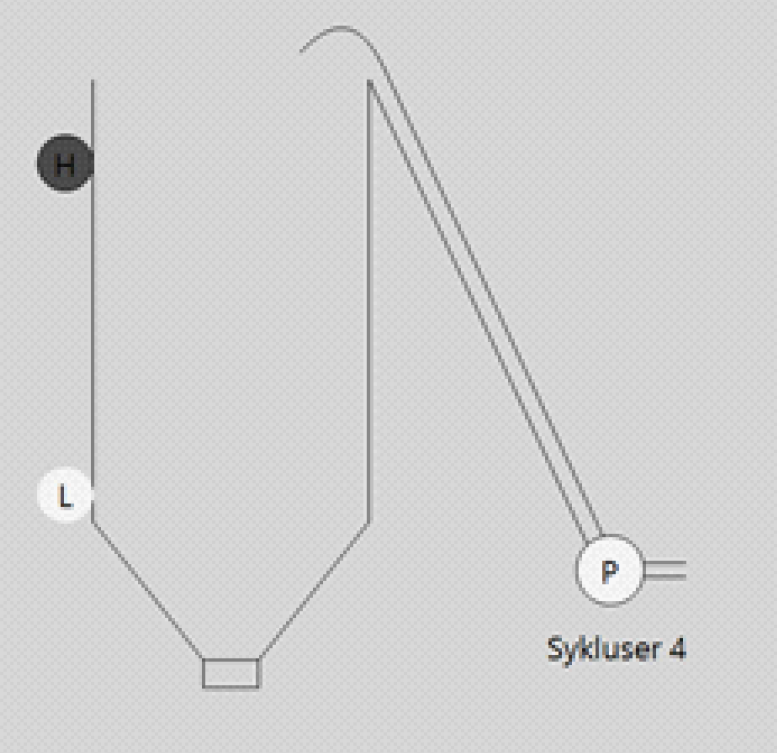
\includegraphics[width=0.5\textwidth]{i08012x01.png}

Der er to nivåvakter i hver silo (L og H) disse gir \textquotedblright{}
TRUE\textquotedblright{} når nivået ligger over giveren.

Virkemåte: Pumpa i en silo skal alltid starte når nivået er under
minimum og stoppe når nivået går over maksimum for siloen.
\begin{enumerate}
\item Lag en Visualisering som ligner den på bildet
\item Anlegget settes i drift med en Start knapp og stoppes med en Stoppknapp.
Når anlegget er satt i drift og nivået er under L startes pumpe P.
Denne går til nivået når H. Slik fortsetter det til driften av anlegget
stoppes.
\item Legg til AutoMan styring av pumpe
\item Legg til en teller for totalt antall sykluser på pumpe (skal vises
på skjerm). 
\item Det skal aktiveres en alarm om det tar mer en 10min (10s) å komme
over L nivå (etter at den har vært under). Alarmen skal ha bekreft
og resett funksjon.
\end{enumerate}

\paragraph{Test oppgave kornsile vanskelig versjon}

Tre kornsiloer skal fyllest ved hjelp av hver sin pumpe P1, P2 og
P3. 

\begin{table}[]
\begin{centering}
\begin{tabular}{|c|c|c|c|}
\hline 
Tilkoblet utstyr & IO på RIO & Variabel & Beskrivelse av tilkoblet utstyr\tabularnewline
\hline 
\hline 
Start Knapp & Bryter1 & Start & \tabularnewline
\hline 
Stopp Knapp & Bryter2 & Stopp & \tabularnewline
\hline 
H Sensor & Bryter3 & LevelHigh & \tabularnewline
\hline 
L Sensor & Bryter4 & LevelLow & \tabularnewline
\hline 
Drifts Lys & Lys1 & Drift & \tabularnewline
\hline 
Pumpe Lys & Lys2 & Pumpe & \tabularnewline
\hline 
Alarm Lys & Lys3 & AlarmLys & \tabularnewline
\hline 
Alarm Lyd & Lys4 & AlarmLyd & \tabularnewline
\hline 
\end{tabular}
\par\end{centering}
\caption{IO-liste for oppkobling mot Gand RIO-trainer}
\end{table}

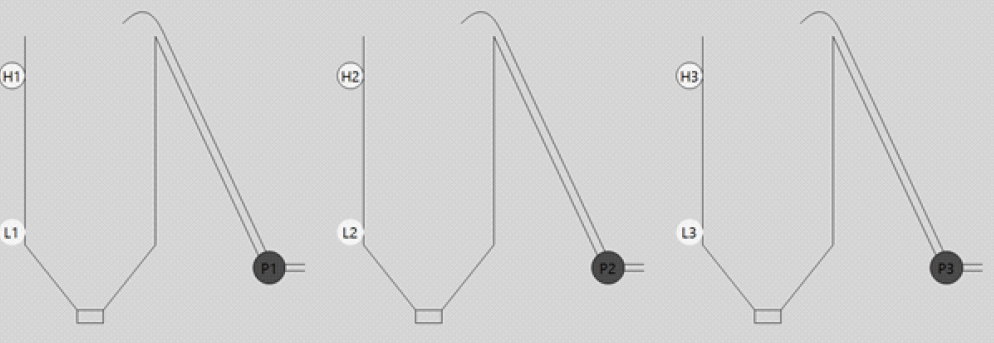
\includegraphics[width=1\textwidth]{i08012x02.png}

Der er to nivåvakter i hver silo (L1, H1, L2. osv.) og alle disse
gir\textquotedblright{} 1\textquotedblright{} når nivået ligger over
giveren. Pumpa i en silo skal alltid starte når nivået er under minimum
og stoppe når nivået går over maksimum for siloen.

Pumpene skal styras slik at det ikke blir brukt mer enn 2000W (P1=500W,
P2=1000W og P3=1500W). Ved tom tank, skal silo fyllest slik at den
ikke lenger er tom (uavhengig av strømforbruk). Alle nettverk programmeres
i LD/FBD. Det skal være mulighet for manuell styring av pumper. 
\begin{enumerate}
\item Anlegget settes i drift med en Start knapp og stoppes med en Stoppknapp.
Når anlegget er satt i drift og nivået er under L startes pumpe P.
Denne går til nivået når H. Dette gjeler for alle pumpene. Slik fortsetter
det til driften av anlegget stoppes. 
\item Komplementer anlegget med alarm dersom nivået ligger under minimum
i mer enn 1 minutt i en av siloene. Alarmsignalet skal pulsere (blinke)
med en frekvens på 1 HZ. 
\item Det er ønskelig med teller for antall sykluser og driftstimer på hver
pumpe. Driftstid og antall sykluser skal presenteres ved hver pumpe.
Når en pumpe kommer over 1000 sykluser eller 1000 driftstimer skal
det vis et varsel om vedlikehold. Dette skal kunne resettes etter
utført vedlikehold. 
\item Sett opp kommunikasjon med Gand-RIO Trainer i henhold til tilordningslisten.
\end{enumerate}
\vskip 10pt
\underbar{file i08012}
\vskip 10pt \filbreak 





\svar{} 
Det er ikke svar på denne oppgave
\vskip 10pt \filbreak 





\notes{} 


%INDEX% PLC, programming, kombinatorisk 

\vfil \eject 




\end{document}
